% *********************************************************************
% © 2026 Jeremy Sylvestre
%
% Permission is granted to copy, distribute and/or modify this document
% under the terms of the GNU Free Documentation License, Version 1.3 or
% any later version published by the Free Software Foundation; with no
% Invariant Sections, no Front-Cover Texts, and no Back-Cover Texts. A
% copy of the license is included in the appendix entitled “GNU Free
% Documentation License” that appears in the output document of this
% PreTeXt source code. All trademarks™ are the registered® marks of
% their respective owners.
%
% *********************************************************************
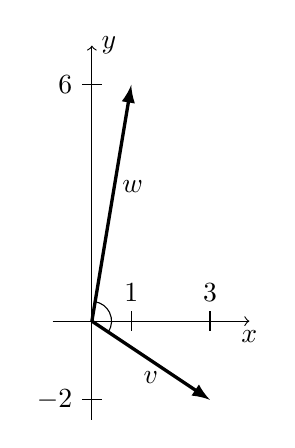
\begin{tikzpicture}[
	vector/.style={-latex,very thick},
	scale=0.5
]
	\draw[->] (-1,0) to (4,0) node[below] {$x$};
	\draw[->] (0,-2.5) to (0,7) node[right] {$y$};

	\draw[vector] (0,0) to node[below] {$\uvec{v}$} (3,-2);
	\draw[thin] (3,-0.25) to (3,0.25) node[above] {$3$};
	\draw[thin] (0.25,-2) to (-0.25,-2) node[left] {$-2$};

	\draw[vector] (0,0) to node[above right] {$\uvec{w}$} (1,6);
	\draw[thin] (1,-0.25) to (1,0.25) node[above] {$1$};
	\draw[thin] (0.25,6) to (-0.25,6) node[left] {$6$};

	% angle arc
	\draw (0,0) ++(-33.69:0.5cm) arc (-33.69:80.538:0.5cm);

\end{tikzpicture}
